\documentclass[preprint,12pt]{elsarticle}
\usepackage[T1]{fontenc}
\usepackage[utf8]{inputenc}
\usepackage{amsmath,amssymb}
\usepackage{graphicx}
\usepackage{booktabs}
\usepackage{adjustbox}
\usepackage{longtable}
\usepackage{lineno}
\usepackage[hidelinks]{hyperref}
\usepackage{xurl}
\biboptions{sort&compress}
\providecommand{\tightlist}{\setlength{\itemsep}{0pt}\setlength{\parskip}{0pt}}
\DeclareUnicodeCharacter{03C9}{\ensuremath{\omega}}
\DeclareUnicodeCharacter{0394}{\ensuremath{\Delta}}
\DeclareUnicodeCharacter{03A3}{\ensuremath{\Sigma}}
\DeclareUnicodeCharacter{03C0}{\ensuremath{\pi}}
\DeclareUnicodeCharacter{2265}{\ensuremath{\geq}}
\DeclareUnicodeCharacter{2264}{\ensuremath{\leq}}
\DeclareUnicodeCharacter{00D7}{\ensuremath{\times}}
\DeclareUnicodeCharacter{2212}{\ensuremath{-}}
\DeclareUnicodeCharacter{00B0}{\ensuremath{^\circ}}
\DeclareUnicodeCharacter{00B2}{\ensuremath{^2}}
\DeclareUnicodeCharacter{2248}{\ensuremath{\approx}}
\DeclareUnicodeCharacter{2192}{\ensuremath{\rightarrow}}
\journal{Renewable Energy}

\begin{document}

\begin{frontmatter}

\title{Energy gain and drivetrain torque exposure of a vortex-generator retrofit: a field assessment at an operating wind farm}

\author{Yi Wang}
\ead{jefflsxy@lsu.edu.cn}
\affiliation{organization={College of Engineering, Lishui University},
            city={Lishui},
            postcode={323000},
            state={Zhejiang},
            country={China}}

\begin{abstract}
Aerodynamic retrofits such as vortex generators are validated by the energy they add, while the extra load they pass to the drivetrain is rarely measured on commercial turbines. At the Hill of Towie wind farm (21 Siemens SWT-2.3-VS-82 turbines), one turbine received vortex generators in September 2021 while the other 20 stayed unmodified for nine months. From open 10-minute SCADA data we estimated the retrofit's effect on energy, time at rated power and a quasi-static main-shaft torque exposure index, comparing the turbine with its own pre-retrofit behaviour in the same farm state and correcting for the drift of 20 placebo turbines. Energy rose by 4.8\% (95\% CI 3.3--6.6\%, joint farm bootstrap), consistent with the operator's independent 4.3\%, time at rated power by 1.7 percentage points (0.7--2.8) and the torque exposure index by 2.3\% (1.6--3.5\%) for an S-N exponent of 3. The exposure ratio, the relative change in torque exposure per relative change in energy, was 0.48 (0.41--0.60), falling to 0.20 for an exponent of 10. Pseudo-retrofit dates and placebo turbines show that the time-at-rated effect is far outside the null range, whereas the energy and exposure effects exceed about 95\% of it. The exposure ratio lies below the value for pure power scaling (0.79) because most of the gain arose at part load and rotor speed absorbed about a third of it. The index measures 10-minute load level, not fatigue damage.
\end{abstract}

\begin{highlights}
\item One retrofitted turbine and 20 unmodified neighbours form a natural experiment
\item Vortex generators raised energy by 4.8\% and time at rated power by 1.7 pp
\item A 10-min torque exposure index rose 0.48\% per 1\% of extra energy (m = 3)
\item Part-load gains and a rotor-speed response keep this below pure power scaling
\item Placebo turbines, pseudo-retrofit dates and injected effects bound the evidence
\end{highlights}

\begin{keyword}
Wind turbine retrofit \sep vortex generators \sep drivetrain loads \sep SCADA \sep natural experiment \sep placebo analysis
\end{keyword}

\end{frontmatter}

\linenumbers

\section{Introduction}

Raising the output and extending the life of the existing fleet is one of the open problems of wind energy \cite{veers19}, and retrofitting operating turbines with aerodynamic add-ons is now a routine way to do the former. Vortex generators (VGs) delay separation on the thick inboard airfoils, raise lift near stall and are typically sold on an annual energy production (AEP) uplift of a few percent \cite{lin02,zhao,mueller,baldacchino18,skrzypinski14}. Field verification of such upgrades has matured into a small methods literature: post-upgrade production is compared with a model of what the turbine would have produced without the upgrade, built from nearby reference turbines or pre-upgrade behaviour \cite{astolfi18,astolfi19,terzi,castellani}, or from statistical models that match pre- and post-upgrade periods on wind and weather covariates \cite{lee15,shin18,latiffianti22}. Power-curve-based assessments must contend with the sensitivity of output to shear, turbulence and atmospheric stability \cite{wagner09,stmartin16} and with the choice and resolution of the SCADA variables used \cite{gonzalez19,astolfi21}. Reported VG uplifts range from about 2\% to 6\% \cite{astolfi18,manolesos,moon,hwangbo17}, and the operator of the Hill of Towie wind farm in Scotland has published an open-source, IEC 61400-12-1-style \cite{iec} validation of its own ``AeroUp'' VG retrofit at +4.3\% (90\% CI 3.3--5.3\%) for the first retrofitted turbine \cite{clerc}.

The other side of the ledger has received far less attention. More energy captured below rated power means more aerodynamic torque passed through the main shaft, gearbox and generator for a larger share of the time. The drivetrain, and the gearbox in particular, already dominates downtime per failure in field reliability surveys \cite{ribrant,tavner07,spinato,faulstich11,pinar,carroll16,artigao}, and its design and failure modes remain an active research topic \cite{nejad22}. Upgrade studies acknowledge that a retrofit may affect the residual lifetime of the turbine \cite{astolfi19}, yet none quantifies the load side. Load effects of VGs are known mainly from aeroelastic simulation, which reports blade-root flapwise damage-equivalent loads (DELs) rising by 4--7\% when VGs are added to contaminated blades \cite{kim}, and from one instrumented research turbine, where VGs on clean blades increased flapwise blade moments \cite{bak}. Multi-criteria retrofit evaluation frameworks call for load metrics but have so far been illustrated with assumed numbers \cite{ji}. Methods that estimate loads from SCADA data exist, but they rely on site-specific aeroelastic simulations or strain-gauge campaigns to train the mapping from SCADA to loads \cite{noppe18,veratudela17,dimitrov18}. To our knowledge no study has measured on commercial turbines how much additional drivetrain torque exposure accompanies the energy gain of an aerodynamic retrofit.

Routine 10-minute SCADA data cannot resolve the load cycles that drive gear and bearing fatigue, but they do record the level of drivetrain torque and how often each level occurs. We therefore ask a narrower question that the data can answer: by how much does a retrofit raise the quasi-static torque exposure of the drivetrain per unit of energy gained? We summarise the answer in an exposure ratio,

\begin{equation}
C = D_{m} / E ,
\label{eq:C}
\end{equation}

the relative change in a power-law-weighted mean of the 10-minute torque (Section 3.1) per relative change in energy. C is a measure of load level, not of fatigue damage or remaining life; translating it into damage requires component-level load and S-N information that SCADA data do not contain.

The Hill of Towie open dataset \cite{hot} makes the comparison possible. Its 21 identical Siemens SWT-2.3-VS-82 turbines were retrofitted in two stages: one turbine (T13) in September 2021, the remaining 20 between July 2022 and May 2023. For nine and a half months one turbine carried the upgrade while 20 sister turbines in the same wind field did not. This is a natural experiment with one treated unit, the setting for which comparative case-study methods with placebo-based inference were developed in econometrics \cite{abadie10,abadie21,conley11}; field campaigns on wake steering at commercial wind farms have used similar toggled or side-by-side designs \cite{fleming19}. The later rollout provides a further, weaker check because no unmodified reference turbines remain.

This paper makes three contributions. (i) We estimate the change in energy, time at rated power and a quasi-static main-shaft torque exposure index caused by the VG retrofit, and we bound the strength of this single-turbine evidence with placebo turbines, pseudo-retrofit dates, injected known effects and a farm-wide joint bootstrap. (ii) We report the exposure ratio C and where in the operating envelope the energy gain and the exposure arise. (iii) We compare the measured C with counterfactuals that add, one at a time, the measured location of the gain and the rotor-speed response of the controller to a pure scaling of power, which shows how much of C these two features explain. The estimator and the tests it had to pass were fixed and time-stamped with SHA-256 hashes before they were run (Section 3.9); two deviations forced by the data are reported as such (Section 3.7).

\section{Data}

\subsection{Site and turbines}

Hill of Towie is an onshore wind farm in Moray, Scotland, owned by TRIG and operated by RES. It comprises 21 Siemens SWT-2.3-VS-82 turbines (rated power 2300 kW, rotor diameter 82 m, geared drivetrain, variable speed, pitch regulated). The turbines entered commercial operation in May 2012, so they were about 9.4 years old when the first retrofit was installed. The operator released 10-minute SCADA data from 2016 onward, alarm logs, a shutdown-duration table and the AeroUp installation dates under a CC BY 4.0 licence \cite{hot}. We use the yearly archives for 2020--2023.

\subsection{The retrofit}

AeroUp is a vortex-generator retrofit \cite{clerc}. T13 was retrofitted on 23--29 September 2021. Works on the other 20 turbines started between 14 July and 20 September 2022; twelve were completed within weeks, eight (T06, T07, T10, T11, T12, T15, T16, T20) only in April--May 2023 (Table 1). A separate control upgrade (TuneUp) was installed on nine turbines in March 2024, outside our analysis windows.

\subsection{Variables}

From tables tblSCTurGrid, tblSCTurbine and tblSCTurTemp we use the 10-minute mean active power P, main-shaft speed n, nacelle yaw position, the power reference set-point, the within-period standard deviation of active power, ambient temperature, and all bearing, gearbox-oil and generator temperature channels. Time stamps mark the end of each 10-minute period; the shutdown table, which marks the start, is shifted by 10 minutes before merging.

\subsection{Normal-operation filter}

A record is kept when the shutdown duration is zero, P \textgreater{} 0, the power set-point is ≥ 2290 kW (no curtailment), and main-shaft speed is above 0.3 rad/s. Across 2020--2023 the filter keeps 72\% of records (Table S1). Records with P ≤ 0 account for most of the loss (15--22\% per year), followed by a reduced power set-point or low rotor speed (4--11\%) and shutdowns (3--7\%). T13 keeps 75--86\% per year. Two turbines, T16 (13--25\%) and T17 (34--53\%), were often run with a reduced set-point; they remain in the placebo fleet, whose median is insensitive to them.

\section{Methods}

\subsection{Outcomes}

For each kept record we form the electrical torque proxy at the main shaft,

\begin{equation}
T = P/\omega , \qquad \omega = 2\pi n/60
\label{eq:T}
\end{equation}

which equals the aerodynamic torque minus drivetrain losses and inertial terms; at 10-minute resolution the inertial term averages out. Outcomes for a target turbine over a window are:

\begin{itemize}
\item
  \emph{E}, the energy ratio change: \(E = \sum P_\mathrm{obs} / \sum P_\mathrm{exp} - 1\);
\item
  \emph{R}, time at rated power: the share of records with P ≥ 0.95 × 2300 kW (in percentage points);
\item
  \(D_{m}\), the torque exposure index for exponent \(m\): \(D_{m} = \left( \overline{T_\mathrm{obs}^{\,m}} \big/ \overline{T_\mathrm{exp}^{\,m}} \right)^{1/m} - 1\), for m = 3, 10/3, 4, 6 and 10;
\item
  \emph{W}, the relative change in mean rotor speed; \(T_1\), the relative change in mean torque; \emph{SD}, the relative change in mean within-10-minute power standard deviation; and temperature residuals for every bearing and gearbox channel.
\end{itemize}

\(D_{m}\) has the form of a damage-equivalent load \cite{burton11} computed from 10-minute means: the exponent weights high-torque periods as a power-law S-N curve would, with m = 3 conventional for shafts and welded structures, 10/3 for roller bearings \cite{iso281}, and 6--10 for gear teeth \cite{nejad14}. It describes the distribution of the quasi-static torque level only. It contains no load cycles within the 10-minute period, no dynamic amplification and no component-specific stress, so it is not a fatigue damage estimate, and changes in \(D_{m}\) cannot be converted into damage or remaining life without further information.

\subsection{Counterfactual from reference turbines}

For each 10-minute stamp we form a farm reference state from all other turbines that are operating normally (at least 10 needed): their mean power, binned in 50 kW steps, and their circular-mean yaw, binned in eight 45° sectors. A target turbine's expected outcome in a post-retrofit record is the mean of its own pre-retrofit records in the same cell (Fig. 1b). Effects are observed minus expected, averaged over post records. This ``reference-cell'' estimator is a discretised version of the side-by-side methods used in upgrade validation \cite{astolfi18,clerc}; it needs no anemometer and no power-curve model, and it treats any change in the target turbine's behaviour relative to its neighbours as the effect. At least 99.4\% of post records fell in a cell populated in the pre window for every turbine (99.95\% for T13).

\subsection{Drift correction (T13 window)}

Pre window: 1 January 2020 -- 22 September 2021; post window: 30 September 2021 -- 13 July 2022. T13 is excluded from every reference set. Each of the 20 unmodified turbines is run through the same estimator with the real dates; because nothing changed on them, their effects measure the estimator's null drift over the same calendar windows (seasonal mix, ageing, wake changes). The drift-corrected T13 effect is the T13 effect minus the median of the 20 placebo effects.

\subsection{Uncertainty and inference}

We use three complementary measures, because no single one covers every source of error in a one-turbine design.

\emph{Joint farm bootstrap.} Each of 1000 draws resamples calendar weeks of the pre and post windows with replacement, the same weeks for all turbines, so that the dependence between turbines and the serial correlation within weeks are preserved \cite{kunsch89,bertrand04}. Within each draw the reference cells, all 21 turbine effects, the placebo median, the corrected E, R, \(D_{m}\) and C, and T13's rank are recomputed. Percentile intervals from these draws are reported as 95\% CIs. They describe sampling variability in time; they do not describe how much an individual turbine's drift can differ from the placebo median.

\emph{Placebo calibration.} To cover that second source we subtract each placebo turbine's own corrected effect from T13's corrected effect, which gives 20 values of what T13's estimate would be if its null drift were like that of each unmodified turbine. Their range is reported as a placebo-calibrated interval, in the spirit of inference from the distribution of control-unit effects when only one unit is treated \cite{conley11}.

\emph{Rank and pseudo-retrofit dates.} T13's rank among the 21 turbines is the placebo permutation test of comparative case studies \cite{abadie10}, for a design in which any turbine could have been the one retrofitted first; under that assumption of exchangeability, rank 1 corresponds to a one-sided p = 1/21 ≈ 0.048. Exchangeability is plausible for identical turbines with the same control system in the same farm, but T13 was not chosen at random, and a turbine-specific trend would violate it. We therefore also apply the full estimator, with the same drift correction, at five pseudo-retrofit dates inside the pre-retrofit period (1 July, 1 September and 1 November 2020, 1 January and 1 March 2021; pre window from 1 January 2020 to eight days before the date, post window up to 290 days after it and no later than 22 September 2021), treating every turbine in turn as the retrofitted one. The resulting 105 turbine-date effects form a null distribution in time and space against which T13's real effect is compared. The pseudo-date windows are shorter than the real ones, so this null is, if anything, wider than the null of the real design.

\subsection{Known-truth checks}

We inject a known effect, post-window power multiplied by 1.04 and capped at 2300 kW with torque scaled at the measured speed, (a) into each of the 20 unmodified turbines over the real windows, and (b) into T13's own data at each pseudo-retrofit date. The estimator, with drift correction, is re-run and the recovered effect is compared with the injected truth computed directly from the altered data. Check (a) tests bias across turbines; check (b) tests recovery on the target turbine itself.

\subsection{Counterfactual decomposition of C}

If a retrofit simply multiplied power by a constant k below the rated cap, at unchanged rotor speed, C would follow from the turbine's own power distribution. Starting from this pure-scaling benchmark (k = 1.05) on T13's pre-retrofit records, we add two features of the observed response one at a time: (b) the measured gain profile, i.e.~T13's drift-corrected relative power uplift in each 200 kW bin of farm reference power, applied record by record at unchanged rotor speed; and (c) the same profile with the rotor speed of region-2 records (P \textless{} 0.9 × rated and speed below 98\% of rated speed) raised by \((1+u)^{1/3}\), the response of a \(K\omega^2\) torque law to a power uplift u. The difference between counterfactual (c) and the measured C is the part that these two features do not explain.

\subsection{Rollout check (deviation D1) and its null (deviation D2)}

The frozen plan specified a replication using turbines not yet retrofitted as references. The installation file showed that works on all 20 turbines started within ten weeks and eight finished only in 2023, so no such reference set exists (deviation D1, recorded before the replication was run). We instead used T13, whose state was constant after 2021, as the single reference turbine: cells are T13 power (50 kW) × T13 yaw (8 sectors); pre = 1 October 2021 -- 13 July 2022 (only T13 retrofitted), post = June, July and October--December 2023 (all retrofitted; August--September dropped because the pre window lacks them); pre records are re-weighted to the post month mix. The pooled effect is the mean over turbines with a turbine-level bootstrap CI. Because all 20 turbines share the same reference turbine and the same year-on-year change, these are not 20 independent replications; the check tests whether the direction and size of the effect recur, not its causal attribution.
Because a single reference turbine is noisier and the windows are a year apart, we added a known-null check after the rollout check had been run (deviation D2): the identical estimator applied to 2020 versus 2021 (same months, no turbine changed state; T13 excluded), with T01 and, separately, T21 as reference. Its pooled effects measure the design's year-on-year drift. The gate for this check was written before it was run.

\subsection{Sensitivity analyses and concurrent-change screen}

One factor at a time from the default: power-bin width (25, 100 kW), yaw sectors (4, 12), minimum number of reference turbines (8, 15), rated threshold (0.90, 0.98 × rated), month-of-year re-weighting of the pre window, dropping the first month after the retrofit, and starting the pre window in October 2020. We also replace the placebo median by the mean and by a trimmed mean, and the reference-power cells by cells of reference-turbine mean nacelle wind speed (0.5 m/s × eight yaw sectors). To screen for changes made to T13 at the same time as the retrofit, we track monthly control signatures of every turbine relative to the fleet median (99th percentile and median rotor speed at rated power, mean power at rated, share of records with a reduced power set-point, median pitch at part load, and the ratio of the nacelle anemometer reading to the fleet median), compare the step in each signature across the retrofit date with the steps of the other 20 turbines, and count alarm-log entries around the works.

\subsection{Staged freezing and code}

The study proceeded in fixed stages, each frozen with a SHA-256 hash before it was run. A baseline script (raw T13 effect with placebo checks) was frozen before its first run. After its result was known, a plan with four pass/fail tests and one informational check was frozen before any of them was run: K1 known truth (Section 3.5a), K2 drift-corrected T13 effect with rank test (Sections 3.3--3.4), K3 rollout check (Section 3.7), K4 seasonal re-weighting, and K5 within-10-minute variability (informational). All four pass/fail tests passed, K3 after the deviations D1 and D2. The plan was time-stamped internally, not publicly registered. The joint bootstrap, placebo calibration, pseudo-retrofit dates, injection into T13, the counterfactual decomposition, the power-bin and wind-speed decompositions, the monthly contrasts and the concurrent-change screen are descriptive analyses added afterwards. The frozen scripts, their hashes and all analysis code are publicly available (see Data and code availability).

\section{Results}

\subsection{Data}

After filtering, 3,069,135 turbine-records of normal operation remain from 4,338,962 merged records for 2020--2023 (median 158,635 per turbine). In the T13 window the pre and post periods contain about 71,800 and 33,400 T13 records.

\subsection{Effects on T13}

Relative to its own pre-retrofit behaviour in the same farm state, T13 produced 3.6\% more energy after the retrofit, spent 1.35 percentage points (pp) more time at rated power, and its torque exposure index (m = 3) rose by 1.75\% (raw estimates). Over the same calendar windows the 20 unmodified turbines drifted in the opposite direction: 17 of 20 show negative energy changes (median −1.2\%), and 18 of 20 show negative time-at-rated changes (Fig. 2). Subtracting the placebo median, the drift-corrected effects on T13 are (Table 2; 95\% CIs from the joint farm bootstrap):

\begin{itemize}
\item
  energy +4.8\% (3.3--6.6\%), consistent with the operator's independent +4.3\% (90\% CI 3.3--5.3\%) \cite{clerc};
\item
  time at rated power +1.67 pp (0.65--2.80);
\item
  torque exposure index +2.3\% for m = 3 (1.6--3.5\%), +2.1\% for m = 10/3 (1.5--3.3\%) and +0.96\% for m = 10 (0.60--1.44\%);
\item
  mean rotor speed +1.66\% (1.12--2.26\%) and mean torque +4.0\% (2.8--5.5\%).
\end{itemize}

T13 ranks first of the 21 turbines on energy, time at rated and exposure in the full sample, and in 79\%, 93\% and 91\% of the joint bootstrap draws, respectively; the corrected effects are positive in every draw.

T13's month-by-month deviation from the fleet has a seasonal pattern of its own (Fig. S4): before the retrofit it ran a few percent below its average in summer and above it in winter. To remove this, Fig. 3 compares each month with the same calendar month one year earlier and subtracts the fleet median of the same difference. In the eight complete pre-retrofit months of 2021 this year-on-year contrast averages −0.7\% for energy, −0.42 pp for time at rated and −0.02\% for torque exposure, with signs scattered around zero. In all nine post-retrofit months it is positive for energy and exposure, averaging +4.1\%, +1.59 pp and +2.2\% respectively, which reproduces the window estimate and gives C = 0.54. Single months are noisy (pre-retrofit months range from −5\% to +6\% in energy), so the evidence lies in the consistent sign after the retrofit rather than in any one month. Re-weighting the pre window to the post-window month mix changes the window estimate only slightly (energy +4.7\%, time at rated +1.42 pp, C = 0.50; Fig. S2).

\subsection{How strong is the single-turbine evidence?}

The three null references in Section 3.4 agree on an ordering: the time-at-rated effect is far outside the null, the energy and exposure effects lie at its upper edge (Fig. 6).

\emph{Placebo calibration.} The corrected effects of the 20 unmodified turbines, which should be zero, have a standard deviation of 1.6\% in energy, 0.26 pp in time at rated and 0.67\% in the exposure index. T13's corrected effects are 3.0, 6.5 and 3.4 of these standard deviations, respectively. Subtracting each placebo's corrected effect from T13's gives placebo-calibrated intervals of 2.2--7.7\% for energy, 1.17--2.14 pp for time at rated and 1.2--3.6\% for exposure; none includes zero. Rotor speed is weaker (−0.3\% to +3.3\%; rank 2 of 21).

\emph{Pseudo-retrofit dates.} Across the 105 turbine-date pairs, the null effects have a 95th percentile of 4.6\% for energy, 0.45 pp for time at rated and 2.2\% for exposure (Fig. 6). T13's real effects exceed 96\% (energy), 100\% (time at rated, null maximum 0.65 pp) and 95\% (exposure) of them. All four null values above T13's energy effect come from T15, T16 and T17; T16 and T17 have by far the lowest share of normal-operation records (13--53\%, Table S1). Without these three turbines the null 95th percentiles are 2.7\% for energy and 1.0\% for exposure, and no null value reaches T13's energy effect. T13 itself, at the five pseudo dates, shows effects between −4.1\% and +0.2\% in energy and between −0.84 and +0.02 pp in time at rated; the largest deviations occur for the pseudo date of 1 March 2021, whose six-month post window covers only spring and summer, the seasons in which T13 runs below its average.

\emph{Known truth.} Injected into the 20 unmodified turbines, the +4\% effect is recovered without bias in the median (energy −0.04 pp, time at rated 0.00 pp, exposure −0.01 pp from the truth), but the error of an individual turbine is that turbine's own drift: its standard deviation is 1.8 pp in energy, 0.27 pp in time at rated and 0.7 pp in exposure (Fig. S3). Injected into T13 itself at the pseudo dates, the recovery errors range from −4.3 to +0.2 pp in energy and from −0.84 to −0.04 pp in time at rated, mirroring the null effects at the same dates.

Taken together, the time-at-rated increase is attributable to the retrofit with high confidence. The energy and exposure increases are consistent with it and with the operator's independent 4.3\%, but a turbine-specific drift of up to about 2--3\% in energy cannot be excluded for a single turbine; their magnitudes carry that uncertainty in addition to the bootstrap CIs.

\subsection{Exposure ratio}

Each 1\% of additional energy came with 0.48\% (95\% CI 0.41--0.60) of additional torque exposure at m = 3 (Fig. 5). The ratio falls with the exponent: 0.45 (0.37--0.57) at m = 10/3, 0.40 at m = 4, 0.31 at m = 6 and 0.20 (0.14--0.27) at m = 10. C is more stable than its numerator and denominator because drift in energy and exposure is correlated: the placebo-calibrated values of C(m = 3) lie between 0.44 and 0.59 for 18 of the 20 placebo turbines (range 0.28--0.89). The sensitivity specifications give C(m = 3) between 0.47 and 0.52 (Fig. S2), and cells defined by reference wind speed give 0.50.

\subsection{Where the gain and the exposure arise}

The energy gain is a part-load phenomenon (Fig. 4a). T13's net relative power uplift is 10--11\% for farm reference power of 200--800 kW, 6--7\% at 800--1600 kW, and below 1.2\% above 1800 kW. Farm states with reference power between 200 and 1000 kW contribute 65\% of the energy gain. The torque-cubed gain is shifted to higher power: bins from 600 to 1600 kW each contribute 14--16\% of it (Fig. 4b), because the exponent weights higher torque more. Time at rated power rises because the turbine reaches rated in slightly lower winds, not because it delivers more at rated. Binning on the mean wind speed of the reference turbines gives the same picture: 85\% of the net energy gain falls below 10 m/s (Fig. S5).

Mean rotor speed rose by 1.66\%, or 0.35 of the energy gain, close to the one third expected when a variable-speed controller absorbs a power gain through a \(K\omega^2\) torque law (\(\Delta\omega/\omega = \tfrac{1}{3}\,\Delta P/P\)). The counterfactuals in Fig. 5 show what the location of the gain and this speed response imply for C(m = 3): pure scaling at fixed speed gives 0.79; applying T13's measured gain profile at fixed speed gives 0.67; adding the \(K\omega^2\) speed response gives 0.58; the measured value is 0.48. Of the gap between pure scaling and the measurement (0.31), the location of the gain accounts for about 0.12, the speed response for about 0.09, and about 0.10 remains unexplained by these two features. The pattern is similar at m = 10 (0.50, 0.32, 0.31 and 0.20). The within-10-minute power standard deviation did not change detectably (+1.1\%, −3.1 to +5.7\%; rank 3), and the mean blade-pitch reference rose by 0.21° (0.08--0.34°; rank 1).

\subsection{Concurrent changes on T13}

None of the control signatures shows a change on T13 at the retrofit date that is unusual within the fleet. Comparing October 2021 -- May 2022 with January -- August 2021, T13's step relative to the fleet median ranks 13th of 21 for the 99th-percentile rotor speed at rated power (−0.002 rpm), 19th for the median rotor speed at rated, 14th for mean power at rated (−1.6 kW), 19th for the share of records with a reduced power set-point and 11th for part-load pitch. There is therefore no sign of a change in rated speed, power limit or fine-pitch setting made with the retrofit. The alarm log shows no change specific to T13. Its total alarm count stays near the fleet median before, during and after the works (rank 9--16 of 21 in each window). The codes logged on T13 during the works week also occur on the other turbines in 2020--2023 (the published alarm descriptions cover only a few codes); two of them (8186/8187) first appear on T13 during the works and on T01 and T15 within a day of the start of their own works in 2022, so they mark the works stop. Codes that were more frequent on T13 in 2021 than in 2020 were equally frequent that year on several unmodified turbines. One sparse code (8110) first appeared on T13 three days after the works, but it also occurs in bursts on nine other turbines between 2020 and 2023. The one signature that did change is the nacelle anemometer: relative to the fleet median, T13's reading rose by about 10 percentage points after the retrofit (from +7--17\% to +13--26\% depending on the month), the largest step of the 21 turbines. This is consistent with the retrofit altering the flow at the nacelle anemometer behind the blade roots, but a sensor exchange during the works cannot be excluded. The estimator does not use T13's anemometer, so the effect estimates are not affected, but the shift explains why binning on T13's own wind speed misplaces the gain (Section 5.1).

\subsection{Thermal side evidence}

Temperatures give only weak support. Compared within the same power and ambient-temperature cells, the gearbox high-speed bearing (generator side) warmed by 0.29 K, the largest change among the 21 turbines (rank 1), and the main bearing by 0.47 K (rank 4). Gearbox oil (−0.06 K, rank 15), the intermediate- and high-speed rotor-side bearings and the generator windings show no distinctive change (ranks 3--15). Of 30 temperature channels, T13 ranks first only on the high-speed bearing; at the resolution of a 21-turbine rank test this is what chance alone would produce about once in 21 channels, so we treat the thermal evidence as consistent with, not as confirmation of, a higher drivetrain load.

\subsection{Rollout check}

With T13 as the only reference turbine, the 20 later-retrofitted turbines show pooled changes of +5.2\% energy (3.2--7.5\%), +1.82 pp time at rated (1.50--2.14; 19 of 20 positive) and +2.8\% torque exposure (2.0--3.7\%), giving C = 0.54 (0.31--0.85) (Fig. 7). The known-null check of this design (2020 vs 2021, no turbine changed) is not null for energy and exposure: +1.0\% energy and +1.05\% exposure with T01 as reference, +2.3\% and +1.35\% with T21. Time at rated is close to null (+0.33 and +0.05 pp). Subtracting the null drift gives rollout effects of about +2.9--4.2\% energy, +1.5--1.8\% exposure and +1.5--1.8 pp time at rated, and C ≈ 0.42--0.50. Because the 20 turbines share one reference turbine and one year-on-year change, this is a consistency check rather than 20 independent replications: it supports the direction and size of the time-at-rated effect and a C of the same order, while its energy and exposure magnitudes depend on a drift correction that we can only bracket.

\section{Discussion}

\subsection{Why the exposure ratio is below pure scaling}

Two features of the response account for about two thirds of the gap between the measured C and pure power scaling, and both are visible in the data. First, the location of the gain. Vortex generators act on the thick inboard sections, where they delay stall at the angles of attack typical of moderate winds \cite{zhao,moon}. At Hill of Towie the relative uplift is largest at low and moderate power and vanishes towards rated power, where torque is high and dominates an index that weights torque by \(T^m\). The steeper the exponent, the stronger this dilution, which is why C falls from 0.48 at m = 3 to 0.20 at m = 10. Second, the controller. Below rated speed, a variable-speed turbine tracks its optimal tip-speed ratio with a generator torque law of the form \emph{T} = \(K\omega^2\) \cite{bossanyi00,johnson06,burton11}, so that \emph{P} = \(K\omega^3\), and part of an aerodynamic gain leaves the drivetrain as speed rather than torque: to first order \(\Delta T/T = \tfrac{2}{3}\,\Delta P/P\) and \(\Delta\omega/\omega = \tfrac{1}{3}\,\Delta P/P\). The measured speed increase of 0.35 times the energy gain matches this, although the single-turbine evidence for the speed change is weaker than for energy (rank 2 of 21). The remaining third of the gap is not explained by these two features. Candidates are a change in the torque distribution within each power bin, the small pitch change, and the turbine-specific drift discussed in Section 4.3; with one retrofitted turbine they cannot be separated.

An independent analysis of the same farm places most of the gain at wind speeds of 10--18 m/s \cite{wang}, which for this turbine lies near and above rated. We traced the difference to the wind-speed variable used for binning (Fig. S5). When we bin our per-record effects on the mean nacelle wind speed of the reference turbines, which the retrofit cannot affect, 85\% of T13's net energy gain falls below 10 m/s, 15\% at 10--13 m/s and almost none above 13 m/s; the relative uplift peaks at +9--11\% at 5--8 m/s and fades to zero as the fleet power curve approaches rated (about 2020 kW at 12 m/s and 2290 kW at 17 m/s on this axis). When we bin the same records on T13's own nacelle anemometer, as is usual in single-turbine power-curve analysis \cite{iec}, 71\% of the gain moves to 10--18 m/s and the uplift turns negative below 6 m/s (−11\% to −19\% at 3--5 m/s). A vortex-generator retrofit that lowers output at low wind is not plausible. T13's anemometer reading rose by about 10\% relative to the fleet at the retrofit (Section 4.6), so an axis based on it shifts post-retrofit records to higher wind-speed bins. We therefore read the 10--18 m/s concentration as a property of the target's own anemometer axis rather than as a disagreement about the size of the effect; both analyses find a gain of about 4--5\%. For load assessment the distinction matters, because the farm-state axis places the gain where torque is low.

\subsection{What the exposure ratio can and cannot inform}

C converts a validated energy uplift into a change in the quasi-static torque level that the drivetrain sees: at Hill of Towie, a 4--5\% energy gain came with about a 2\% higher torque exposure index at m = 3 and about 1\% at m = 10. For an owner this is a first-order screening quantity. It shows that the retrofit did not raise the drivetrain's torque level in proportion to the energy, and it can be estimated at no extra cost from the same SCADA data and side-by-side design already used to validate the energy gain \cite{astolfi18,clerc}. It is not a fatigue damage or lifetime estimate. Converting it into damage would require the load cycles within each 10-minute period, the transfer from shaft torque to gear and bearing stresses, and component S-N data, none of which SCADA provides. Turbines with a known gearbox weakness or in life extension are the cases where C should be followed up with such data, for example with high-rate torque or strain measurements on a retrofitted and an unmodified turbine.

\subsection{Limitations}

\begin{itemize}
\item
  \textbf{Quasi-static exposure, not fatigue.} T = P/ω is an electrical torque estimate averaged over 10 minutes. \(D_{m}\) and C describe the torque level and its distribution, not the cycles inside each 10-minute period, which drive much of the gear-tooth and bearing damage. The within-period power standard deviation did not change detectably, which argues against a large change in fluctuation amplitude, but it is not a substitute for strain-gauge or high-rate torque data.
\item
  \textbf{Drivetrain only.} Blade-root and tower loads, the components on which VG studies have reported load increases \cite{kim,bak}, are not observable in SCADA data.
\item
  \textbf{One turbine.} The main estimate rests on a single retrofitted turbine. Its rank of 1 in 21 gives the smallest p-value a 21-turbine permutation can produce, and exchangeability is an assumption (Section 3.4). The pseudo-retrofit null places the energy and exposure effects at about the 95th--96th percentile; a turbine-specific drift of the size seen at some pseudo dates would change their magnitudes by up to 2--4 percentage points in energy.
\item
  \textbf{Rollout check.} The 2022--23 rollout supports the direction of the effect, but its single-reference design carries a year-on-year drift of 1--2\% in energy and about 1.2\% in exposure that we can only bracket (deviations D1 and D2), and its 20 turbines are not independent replications.
\item
  \textbf{Drift of the reference fleet.} The 20 placebo turbines drifted by a median −1.2\% in energy over the T13 window. The correction is robust to the choice of median, mean or trimmed mean, but the cause of the drift (seasonal mix, wake changes, ageing \cite{staffell14}) is not identified.
\item
  \textbf{Concurrent changes.} Control signatures and the alarm log show no change made with the retrofit other than the works themselves, but the nacelle anemometer reading of T13 shifted, and maintenance that leaves no trace in SCADA or alarm data cannot be ruled out.
\item
  \textbf{Mechanism.} Location of the gain and the speed response explain about two thirds of the gap to pure scaling; the rest is unexplained.
\item
  \textbf{Seasonal heterogeneity of T13.} T13 deviates from the fleet seasonally (Fig. S4). The window estimate, the month-re-weighted estimate and the same-month year-on-year contrast agree (energy 4.1--4.8\%, C 0.48--0.54), but a seasonally varying retrofit effect cannot be excluded with one turbine-year of post data.
\end{itemize}

\section{Conclusions}

\begin{itemize}
\item
  A vortex-generator retrofit at an operating wind farm raised energy by 4.8\% (95\% CI 3.3--6.6\%) and time at rated power by 1.7 pp on the first retrofitted turbine, measured against 20 unmodified neighbours. The time-at-rated effect lies far outside the null range of placebo turbines and pseudo-retrofit dates; the energy effect lies at its upper edge and agrees with the operator's independent estimate.
\item
  A quasi-static main-shaft torque exposure index rose by about 0.5\% per 1\% of extra energy at m = 3 and by 0.2\% at m = 10.
\item
  At m = 3 the exposure ratio is about 60\% of what pure power scaling implies. The concentration of the gain at part load and a rotor-speed response consistent with the controller's torque law explain about two thirds of the difference.
\item
  The 2022--23 rollout on 20 further turbines is consistent in direction, with a time-at-rated increase of 1.5--1.8 pp after drift correction.
\item
  The exposure ratio can be estimated from routine SCADA data alongside standard energy-uplift validation. It screens the load-level side of a retrofit; fatigue damage and remaining life require load measurements that SCADA does not provide.
\end{itemize}


\section*{CRediT authorship contribution statement}

\textbf{Yi Wang:} Conceptualization, Methodology, Software, Formal analysis, Data curation, Visualization, Validation, Writing -- original draft, Writing -- review \& editing.

\section*{Declaration of competing interest}

The author declares no known competing financial interests or personal relationships that could have appeared to influence the work reported in this paper.

\section*{Funding}

This research did not receive any specific grant from funding agencies in the public, commercial, or not-for-profit sectors.

\section*{Acknowledgements}

We thank RES and the owners of the Hill of Towie wind farm for releasing the SCADA data, shutdown records and retrofit dates as an open dataset.

\section*{Data and code availability}

The data are the Hill of Towie wind farm open dataset, version 2.1.0, Zenodo, \url{https://doi.org/10.5281/zenodo.22662930} (CC BY 4.0) \cite{hot}. The frozen test scripts with their SHA-256 hashes, the paper analysis scripts and the figure code are available at \url{https://github.com/jeff-1980/aeroup-vg-load-cost}.

\section*{Declaration of generative AI and AI-assisted technologies in the manuscript preparation process}

During the preparation of this work the author used Claude (Anthropic) in order to write analysis code and to draft and edit the text. After using this tool, the author reviewed and edited the content as needed and takes full responsibility for the content of the published article.


\begin{thebibliography}{99}
\bibitem{veers19} P. Veers, K. Dykes, E. Lantz, S. Barth, C.L. Bottasso, O. Carlson, et al., Grand challenges in the science of wind energy, Science 366 (2019) eaau2027. \url{https://doi.org/10.1126/science.aau2027}.
\bibitem{lin02} J.C. Lin, Review of research on low-profile vortex generators to control boundary-layer separation, Prog. Aerosp. Sci. 38 (2002) 389--420. \url{https://doi.org/10.1016/S0376-0421(02)00010-6}.
\bibitem{zhao} Z. Zhao, R. Jiang, J. Feng, H. Liu, T. Wang, W. Shen, M. Chen, D. Wang, Y. Liu, Researches on vortex generators applied to wind turbines: a review, Ocean Eng. 253 (2022) 111266. \url{https://doi.org/10.1016/j.oceaneng.2022.111266}.
\bibitem{mueller} H. Mueller-Vahl, G. Pechlivanoglou, C.N. Nayeri, C.O. Paschereit, Vortex generators for wind turbine blades: a combined wind tunnel and wind turbine parametric study, in: Proc. ASME Turbo Expo 2012: Turbine Technical Conference and Exposition, Vol. 6, Copenhagen, 2012, pp. 899--914. \url{https://doi.org/10.1115/GT2012-69197}.
\bibitem{baldacchino18} D. Baldacchino, C. Ferreira, D. De Tavernier, W.A. Timmer, G.J.W. van Bussel, Experimental parameter study for passive vortex generators on a 30\% thick airfoil, Wind Energy 21 (2018) 745--765. \url{https://doi.org/10.1002/we.2191}.
\bibitem{skrzypinski14} W. Skrzypiński, M. Gaunaa, C. Bak, The effect of mounting vortex generators on the DTU 10MW reference wind turbine blade, J. Phys. Conf. Ser. 524 (2014) 012034. \url{https://doi.org/10.1088/1742-6596/524/1/012034}.
\bibitem{astolfi18} D. Astolfi, F. Castellani, L. Terzi, Wind turbine power curve upgrades, Energies 11 (2018) 1300. \url{https://doi.org/10.3390/en11051300}.
\bibitem{astolfi19} D. Astolfi, F. Castellani, M.L. Fravolini, S. Cascianelli, L. Terzi, Precision computation of wind turbine power upgrades: an aerodynamic and control optimization test case, J. Energy Resour. Technol. 141 (2019) 051205. \url{https://doi.org/10.1115/1.4042450}.
\bibitem{terzi} L. Terzi, A. Lombardi, F. Castellani, D. Astolfi, Innovative methods for wind turbine power curve upgrade assessment, J. Phys. Conf. Ser. 1102 (2018) 012036. \url{https://doi.org/10.1088/1742-6596/1102/1/012036}.
\bibitem{castellani} F. Castellani, D. Astolfi, L. Terzi, Wind turbine power curve upgrades: methods for the assessment and test cases study, J. Phys. Conf. Ser. 1452 (2020) 012004. \url{https://doi.org/10.1088/1742-6596/1452/1/012004}.
\bibitem{lee15} G. Lee, Y. Ding, L. Xie, M.G. Genton, A kernel plus method for quantifying wind turbine performance upgrades, Wind Energy 18 (2015) 1207--1219. \url{https://doi.org/10.1002/we.1755}.
\bibitem{shin18} Y. Shin, Y. Ding, J.Z. Huang, Covariate matching methods for testing and quantifying wind turbine upgrades, Ann. Appl. Stat. 12 (2018) 1271--1292. \url{https://doi.org/10.1214/17-AOAS1109}.
\bibitem{latiffianti22} E. Latiffianti, Y. Ding, S. Sheng, L. Williams, M. Morshedizadeh, M. Rodgers, Analysis of leading edge protection application on wind turbine performance through energy and power decomposition approaches, Wind Energy 25 (2022) 1203--1221. \url{https://doi.org/10.1002/we.2722}.
\bibitem{wagner09} R. Wagner, I. Antoniou, S.M. Pedersen, M.S. Courtney, H.E. Jørgensen, The influence of the wind speed profile on wind turbine performance measurements, Wind Energy 12 (2009) 348--362. \url{https://doi.org/10.1002/we.297}.
\bibitem{stmartin16} C.M. St. Martin, J.K. Lundquist, A. Clifton, G.S. Poulos, S.J. Schreck, Wind turbine power production and annual energy production depend on atmospheric stability and turbulence, Wind Energy Sci. 1 (2016) 221--236. \url{https://doi.org/10.5194/wes-1-221-2016}.
\bibitem{gonzalez19} E. Gonzalez, B. Stephen, D. Infield, J.J. Melero, Using high-frequency SCADA data for wind turbine performance monitoring: a sensitivity study, Renew. Energy 131 (2019) 841--853. \url{https://doi.org/10.1016/j.renene.2018.07.068}.
\bibitem{astolfi21} D. Astolfi, F. Castellani, A. Lombardi, L. Terzi, Multivariate SCADA data analysis methods for real-world wind turbine power curve monitoring, Energies 14 (2021) 1105. \url{https://doi.org/10.3390/en14041105}.
\bibitem{manolesos} M. Manolesos, Y. Celik, H. Ramsay, R. Karande, B. Wood, I. Dinwoodie, I. Masters, M. Harrold, G. Papadakis, Performance improvement of a Vestas V52 850kW wind turbine by retrofitting passive flow control devices, J. Phys. Conf. Ser. 2767 (2024) 022027. \url{https://doi.org/10.1088/1742-6596/2767/2/022027}.
\bibitem{moon} H. Moon, J. Jeong, S. Park, K. Ha, J.-H. Jeong, Numerical and experimental validation of vortex generator effect on power performance improvement in MW-class wind turbine blade, Renew. Energy 212 (2023) 443--454. \url{https://doi.org/10.1016/j.renene.2023.04.104}.
\bibitem{hwangbo17} H. Hwangbo, Y. Ding, O. Eisele, G. Weinzierl, U. Lang, G. Pechlivanoglou, Quantifying the effect of vortex generator installation on wind power production: an academia-industry case study, Renew. Energy 113 (2017) 1589--1597. \url{https://doi.org/10.1016/j.renene.2017.07.009}.
\bibitem{iec} IEC 61400-12-1:2022, Wind energy generation systems -- Part 12-1: Power performance measurements of electricity producing wind turbines, Edition 3.0, International Electrotechnical Commission, Geneva, 2022.
\bibitem{clerc} A. Clerc, A. Torner, A. Bamberger, M. Lannic, E. Lingkan, S. Northover-Naylor, G. Powles, K. Watts, T. Young, Open-source dataset and AEP validation from a real-world case study of turbine upgrades worth 5\% AEP, presentation at WindEurope Technology Workshop 2025, Istanbul, 20 June 2025. https://www.res-group.com/wp-content/uploads/2026/05/RES-open-source-AEP-validation-of-turbine-upgrades.pdf (accessed 1 November 2026).
\bibitem{ribrant} J. Ribrant, L.M. Bertling, Survey of failures in wind power systems with focus on Swedish wind power plants during 1997--2005, IEEE Trans. Energy Convers. 22 (2007) 167--173. \url{https://doi.org/10.1109/TEC.2006.889614}.
\bibitem{tavner07} P.J. Tavner, J. Xiang, F. Spinato, Reliability analysis for wind turbines, Wind Energy 10 (2007) 1--18. \url{https://doi.org/10.1002/we.204}.
\bibitem{spinato} F. Spinato, P.J. Tavner, G.J.W. van Bussel, E. Koutoulakos, Reliability of wind turbine subassemblies, IET Renew. Power Gener. 3 (2009) 387--401. \url{https://doi.org/10.1049/iet-rpg.2008.0060}.
\bibitem{faulstich11} S. Faulstich, B. Hahn, P.J. Tavner, Wind turbine downtime and its importance for offshore deployment, Wind Energy 14 (2011) 327--337. \url{https://doi.org/10.1002/we.421}.
\bibitem{pinar} J.M. Pinar Pérez, F.P. García Márquez, A. Tobias, M. Papaelias, Wind turbine reliability analysis, Renew. Sustain. Energy Rev. 23 (2013) 463--472. \url{https://doi.org/10.1016/j.rser.2013.03.018}.
\bibitem{carroll16} J. Carroll, A. McDonald, D. McMillan, Failure rate, repair time and unscheduled O\&M cost analysis of offshore wind turbines, Wind Energy 19 (2016) 1107--1119. \url{https://doi.org/10.1002/we.1887}.
\bibitem{artigao} E. Artigao, S. Martín-Martínez, A. Honrubia-Escribano, E. Gómez-Lázaro, Wind turbine reliability: a comprehensive review towards effective condition monitoring development, Appl. Energy 228 (2018) 1569--1583. \url{https://doi.org/10.1016/j.apenergy.2018.07.037}.
\bibitem{nejad22} A.R. Nejad, J. Keller, Y. Guo, S. Sheng, H. Polinder, S. Watson, et al., Wind turbine drivetrains: state-of-the-art technologies and future development trends, Wind Energy Sci. 7 (2022) 387--411. \url{https://doi.org/10.5194/wes-7-387-2022}.
\bibitem{kim} S. Kim, H. Im, B. Kim, Numerical analysis of the effects of vortex generators attached to contaminated blades on wind turbine power performance and fatigue load, J. Mech. Sci. Technol. 37 (2023) 3515--3524. \url{https://doi.org/10.1007/s12206-023-0617-0}.
\bibitem{bak} C. Bak, W. Skrzypiński, M. Gaunaa, H. Villanueva, N.F. Brønnum, E.K. Kruse, Full scale wind turbine test of vortex generators mounted on the entire blade, J. Phys. Conf. Ser. 753 (2016) 022001. \url{https://doi.org/10.1088/1742-6596/753/2/022001}.
\bibitem{ji} F. Ji, F. Yang, Z. Wang, S. Liu, D. Xu, W. Zhou, L. Wu, X. Chu, Y. Zhong, Y. Ke, Modular performance testing and comparative evaluation method for wind turbine retrofit schemes, Machines 14 (2026) 965. \url{https://doi.org/10.3390/machines14090965}.
\bibitem{noppe18} N. Noppe, W. Weijtjens, C. Devriendt, Modeling of quasi-static thrust load of wind turbines based on 1 s SCADA data, Wind Energy Sci. 3 (2018) 139--147. \url{https://doi.org/10.5194/wes-3-139-2018}.
\bibitem{veratudela17} L. Vera-Tudela, M. Kühn, Analysing wind turbine fatigue load prediction: the impact of wind farm flow conditions, Renew. Energy 107 (2017) 352--360. \url{https://doi.org/10.1016/j.renene.2017.01.065}.
\bibitem{dimitrov18} N. Dimitrov, M.C. Kelly, A. Vignaroli, J. Berg, From wind to loads: wind turbine site-specific load estimation with surrogate models trained on high-fidelity load databases, Wind Energy Sci. 3 (2018) 767--790. \url{https://doi.org/10.5194/wes-3-767-2018}.
\bibitem{hot} A. Clerc, E. Lingkan, Hill of Towie wind farm open dataset, version 2.1.0 [dataset], Zenodo, 2026. \url{https://doi.org/10.5281/zenodo.22662930}.
\bibitem{abadie10} A. Abadie, A. Diamond, J. Hainmueller, Synthetic control methods for comparative case studies: estimating the effect of California's tobacco control program, J. Am. Stat. Assoc. 105 (2010) 493--505. \url{https://doi.org/10.1198/jasa.2009.ap08746}.
\bibitem{abadie21} A. Abadie, Using synthetic controls: feasibility, data requirements, and methodological aspects, J. Econ. Lit. 59 (2021) 391--425. \url{https://doi.org/10.1257/jel.20191450}.
\bibitem{conley11} T.G. Conley, C.R. Taber, Inference with "difference in differences" with a small number of policy changes, Rev. Econ. Stat. 93 (2011) 113--125. \url{https://doi.org/10.1162/REST_a_00049}.
\bibitem{fleming19} P. Fleming, J. King, K. Dykes, E. Simley, J. Roadman, A. Scholbrock, et al., Initial results from a field campaign of wake steering applied at a commercial wind farm -- Part 1, Wind Energy Sci. 4 (2019) 273--285. \url{https://doi.org/10.5194/wes-4-273-2019}.
\bibitem{burton11} T. Burton, N. Jenkins, D. Sharpe, E. Bossanyi, Wind Energy Handbook, second ed., John Wiley \& Sons, Chichester, 2011. \url{https://doi.org/10.1002/9781119992714}.
\bibitem{iso281} ISO 281:2007, Rolling bearings -- Dynamic load ratings and rating life, International Organization for Standardization, Geneva, 2007.
\bibitem{nejad14} A.R. Nejad, Z. Gao, T. Moan, On long-term fatigue damage and reliability analysis of gears under wind loads in offshore wind turbine drivetrains, Int. J. Fatigue 61 (2014) 116--128. \url{https://doi.org/10.1016/j.ijfatigue.2013.11.023}.
\bibitem{kunsch89} H.R. Künsch, The jackknife and the bootstrap for general stationary observations, Ann. Stat. 17 (1989) 1217--1241. \url{https://doi.org/10.1214/aos/1176347265}.
\bibitem{bertrand04} M. Bertrand, E. Duflo, S. Mullainathan, How much should we trust differences-in-differences estimates?, Q. J. Econ. 119 (2004) 249--275. \url{https://doi.org/10.1162/003355304772839588}.
\bibitem{bossanyi00} E.A. Bossanyi, The design of closed loop controllers for wind turbines, Wind Energy 3 (2000) 149--163. \url{https://doi.org/10.1002/we.34}.
\bibitem{johnson06} K.E. Johnson, L.Y. Pao, M.J. Balas, L.J. Fingersh, Control of variable-speed wind turbines: standard and adaptive techniques for maximizing energy capture, IEEE Control Syst. Mag. 26 (2006) 70--81. \url{https://doi.org/10.1109/MCS.2006.1636311}.
\bibitem{wang} Q. Wang, Y. Vidal, Neighbor-based estimation of wind turbine power for upgrade performance assessment, J. Phys. Conf. Ser. 3232 (2026) 012001. \url{https://doi.org/10.1088/1742-6596/3232/1/012001}.
\bibitem{staffell14} I. Staffell, R. Green, How does wind farm performance decline with age?, Renew. Energy 66 (2014) 775--786. \url{https://doi.org/10.1016/j.renene.2013.10.041}.
\end{thebibliography}

\clearpage
\begin{table}[htbp]
\centering
\caption{AeroUp installation dates (first and last day of works)}
\label{tab:install}
\small
\begin{adjustbox}{max width=\textwidth}
\begin{tabular}{lllllll}
\toprule
Turbine & First & Last &  & Turbine & First & Last \\
\midrule
T01 & 2022-07-23 & 2022-08-01 &  & T12 & 2022-09-01 & 2023-05-09 \\
T02 & 2022-07-18 & 2022-07-28 &  & \textbf{T13} & \textbf{2021-09-23} & \textbf{2021-09-29} \\
T03 & 2022-07-28 & 2022-08-14 &  & T14 & 2022-08-30 & 2022-10-03 \\
T04 & 2022-07-31 & 2022-09-10 &  & T15 & 2022-07-14 & 2023-05-26 \\
T05 & 2022-07-16 & 2022-07-22 &  & T16 & 2022-08-27 & 2023-04-15 \\
T06 & 2022-07-16 & 2023-04-15 &  & T17 & 2022-08-10 & 2022-08-27 \\
T07 & 2022-09-20 & 2023-05-25 &  & T18 & 2022-08-22 & 2022-09-21 \\
T08 & 2022-08-08 & 2022-09-21 &  & T19 & 2022-08-11 & 2022-08-23 \\
T09 & 2022-09-13 & 2022-10-03 &  & T20 & 2022-08-13 & 2023-04-20 \\
T10 & 2022-08-04 & 2023-04-26 &  & T21 & 2022-08-21 & 2022-09-01 \\
T11 & 2022-09-09 & 2023-05-18 &  &  &  &  \\
\bottomrule
\end{tabular}
\end{adjustbox}

\par\smallskip\parbox{0.95\textwidth}{\footnotesize Source: Hill\_of\_Towie\_AeroUp\_install\_dates.csv in the dataset.}
\end{table}

\begin{table}[htbp]
\centering
\caption{Drift-corrected effects on T13}
\label{tab:effects}
\small
\begin{adjustbox}{max width=\textwidth}
\begin{tabular}{lllll}
\toprule
Outcome & Estimate & 95\% CI (joint farm bootstrap) & Placebo-calibrated interval & Rank of 21 \\
\midrule
Energy ratio change & +4.81\% & 3.28 to 6.59\% & 2.22 to 7.66\% & 1 \\
Time at rated power & +1.67 pp & 0.65 to 2.80 & 1.17 to 2.14 & 1 \\
Torque exposure, m = 3 & +2.30\% & 1.57 to 3.54\% & 1.15 to 3.56\% & 1 \\
Torque exposure, m = 10/3 & +2.15\% & 1.45 to 3.34\% & 1.08 to 3.33\% & 1 \\
Torque exposure, m = 4 & +1.93\% & 1.27 to 2.97\% &  & 1 \\
Torque exposure, m = 6 & +1.48\% & 0.92 to 2.20\% &  & 1 \\
Torque exposure, m = 10 & +0.96\% & 0.60 to 1.44\% & 0.51 to 1.53\% & 1 \\
Mean rotor speed & +1.66\% & 1.12 to 2.26\% & $-$0.28 to 3.27\% & 2 \\
Mean torque & +3.98\% & 2.75 to 5.46\% &  &  \\
Pitch reference & +0.21° & 0.08 to 0.34°$^{\mathrm{a}}$ &  & 1 \\
Within-10-min power std & +1.1\% & $-$3.1 to +5.7\%$^{\mathrm{a}}$ &  & 3 \\
C (m = 3) & 0.48 & 0.41 to 0.60 & 0.28 to 0.89$^{\mathrm{b}}$ &  \\
C (m = 10/3) & 0.45 & 0.37 to 0.57 &  &  \\
C (m = 10) & 0.20 & 0.14 to 0.27 & 0.09 to 0.46$^{\mathrm{b}}$ &  \\
\bottomrule
\end{tabular}
\end{adjustbox}

\par\smallskip\parbox{0.95\textwidth}{\footnotesize $^{\mathrm{a}}$ Weekly block bootstrap of T13 with the placebo median held fixed. $^{\mathrm{b}}$ 18 of 20 values between 0.44 and 0.59 (m = 3) and between 0.15 and 0.26 (m = 10).}
\end{table}


\clearpage
\begin{figure}[htbp]
\centering
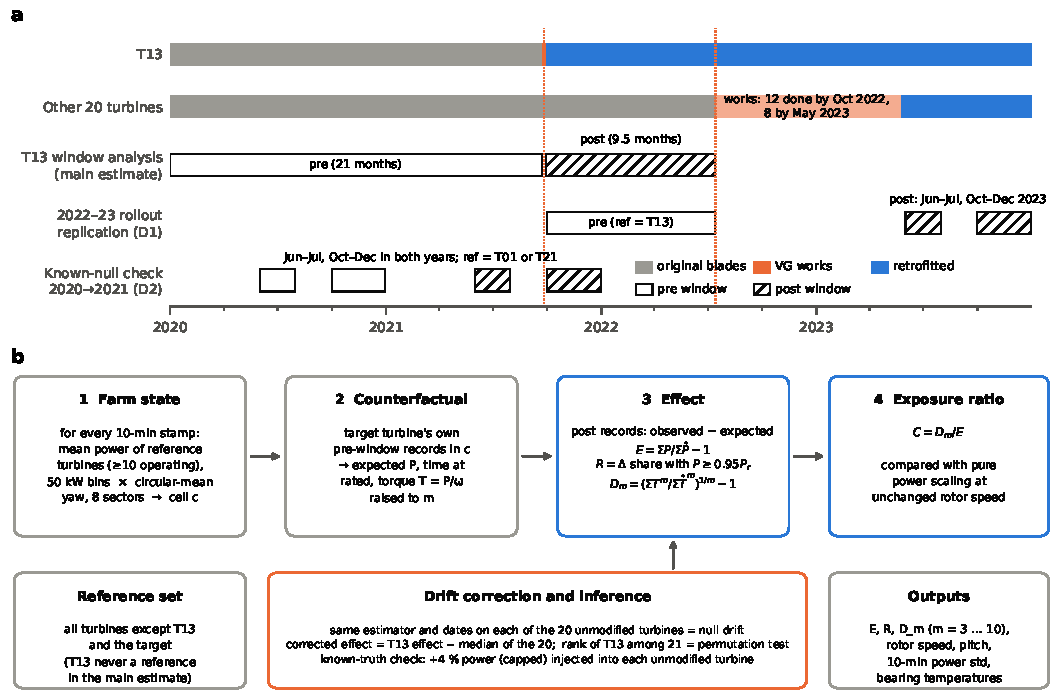
\includegraphics[width=\textwidth]{figures/fig1_design.pdf}
\caption{Study design. (a) Retrofit timeline and analysis windows. T13 received vortex generators on 23--29 September 2021; the other 20 turbines were retrofitted between 14 July 2022 and 26 May 2023. Main estimate: T13 pre window 1 January 2020 -- 22 September 2021, post window 30 September 2021 -- 13 July 2022, with all 20 unmodified turbines as the reference fleet. Rollout check (deviation D1): the 20 later turbines, with T13 as the single reference, comparing October 2021 -- July 2022 with June--July and October--December 2023. Known-null check (deviation D2): the same single-reference design applied to the same calendar months of 2020 and 2021, when no turbine changed. (b) Reference-cell estimator. Each 10-minute stamp is assigned to a farm-state cell (reference mean power × yaw sector); the target turbine's expected outcome is its own pre-window mean in that cell; effects compare observed and expected post-window records; the null drift is measured by running the identical estimator on each unmodified turbine.}
\label{fig:1}
\end{figure}

\begin{figure}[htbp]
\centering
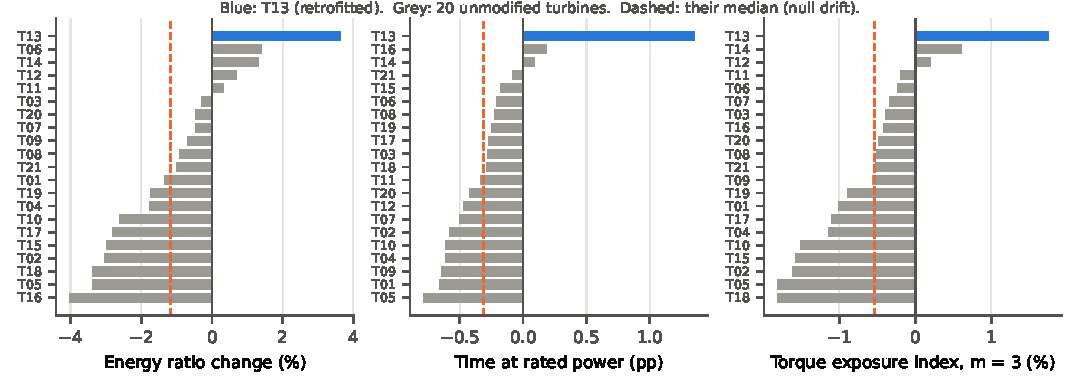
\includegraphics[width=\textwidth]{figures/fig2_per_turbine.pdf}
\caption{Raw effects in the T13 window for all 21 turbines, each estimated against the same reference set (all turbines except T13 and the target). Blue: T13 (retrofitted). Grey: unmodified turbines, whose effects measure the null drift of the estimator; dashed line: their median, which is subtracted to obtain drift-corrected effects.}
\label{fig:2}
\end{figure}

\begin{figure}[htbp]
\centering
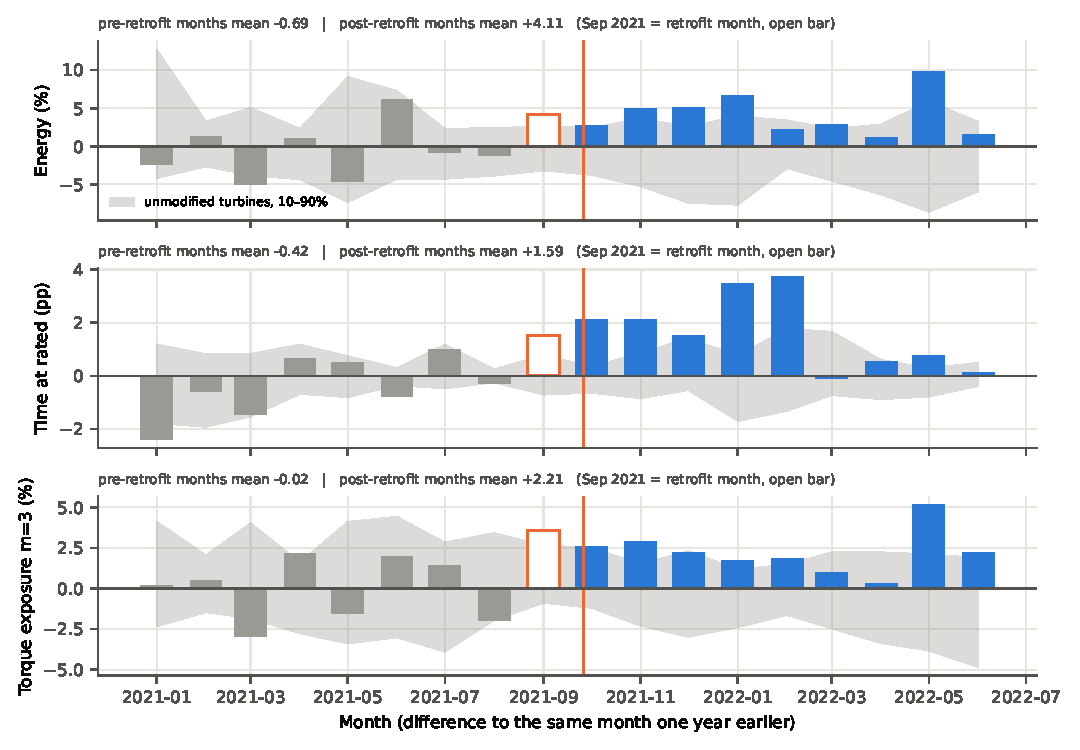
\includegraphics[width=\textwidth]{figures/fig3_event_study.pdf}
\caption{Same-calendar-month year-on-year contrast. Each bar is T13's monthly effect minus its effect in the same month a year earlier, minus the fleet median of the same difference. Grey band: 10th--90th percentile of the unmodified turbines. Open bar: retrofit month (September 2021).}
\label{fig:3}
\end{figure}

\begin{figure}[htbp]
\centering
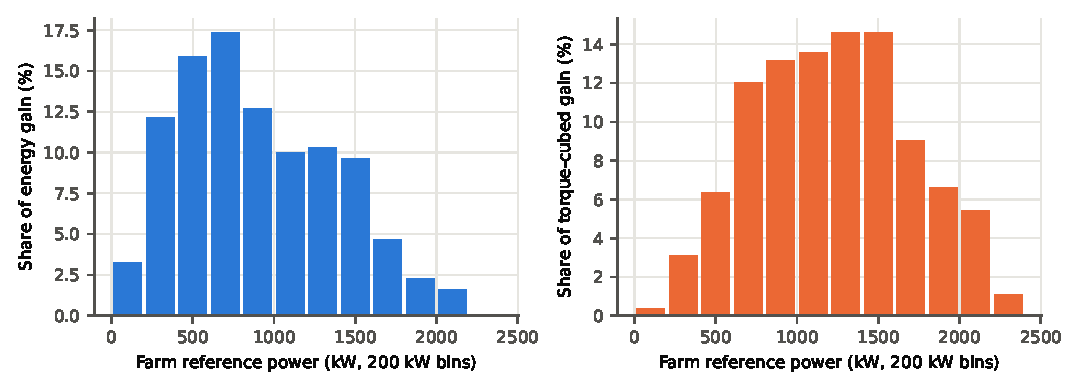
\includegraphics[width=\textwidth]{figures/fig4_power_bins.pdf}
\caption{Where the gain arises. Share of T13's energy gain (a) and of its torque-cubed gain (b) by farm reference power, after subtracting the median of the unmodified turbines.}
\label{fig:4}
\end{figure}

\begin{figure}[htbp]
\centering
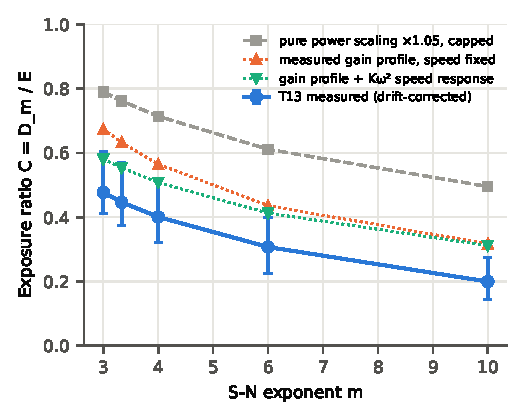
\includegraphics[width=\textwidth]{figures/fig5_cost_ratio.pdf}
\caption{Exposure ratio C = \(D_{m}\)/E against the exponent m. Blue: T13, drift-corrected, with 95\% intervals from the joint farm bootstrap. Grey: pure power scaling (×1.05, capped at rated, rotor speed unchanged) applied to T13's pre-retrofit records. Orange: T13's measured gain profile by farm reference power applied at unchanged rotor speed. Green: the same profile with the region-2 rotor-speed response of a \(K\omega^2\) torque law.}
\label{fig:5}
\end{figure}

\begin{figure}[htbp]
\centering
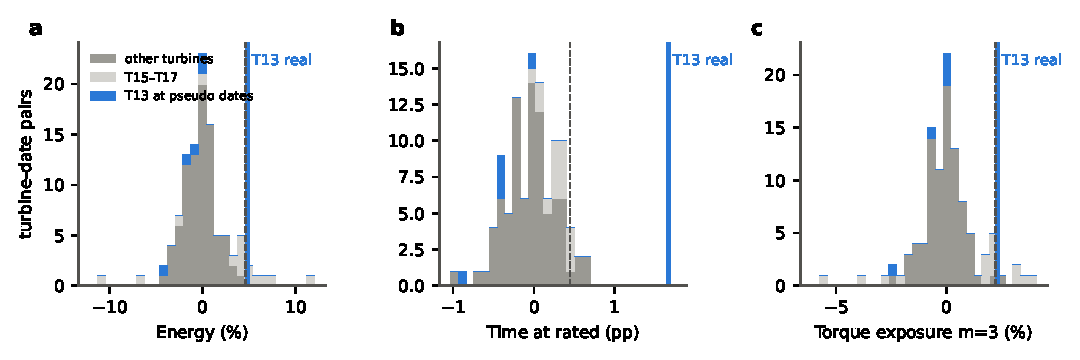
\includegraphics[width=\textwidth]{figures/fig6_null.pdf}
\caption{T13's drift-corrected effects (blue line) against the null distribution from pseudo-retrofit dates inside the pre-retrofit period (five dates × 21 turbines, each corrected by the median of the other 20). Dark grey: turbines other than T13 and T15--T17; light grey: T15--T17; blue bars: T13 at the pseudo dates. Dashed line: 95th percentile of all 105 null values. (a) Energy; (b) time at rated power; (c) torque exposure index, m = 3.}
\label{fig:6}
\end{figure}

\begin{figure}[htbp]
\centering
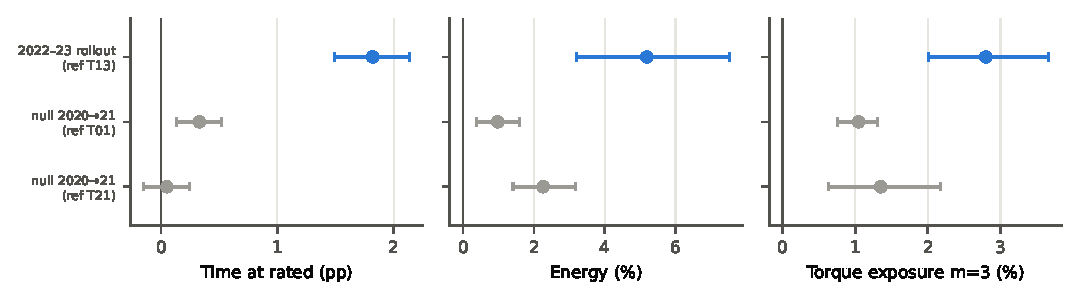
\includegraphics[width=\textwidth]{figures/fig7_replication.pdf}
\caption{Rollout check on the 2022--23 retrofits with T13 as the single reference turbine (blue), and the known-null check of the same design on 2020 versus 2021 with T01 or T21 as reference (grey). Intervals: 95\% turbine bootstrap. The 20 turbines share one reference and are not independent replications.}
\label{fig:7}
\end{figure}


\end{document}
